\section{Remoção}

\begin{frame}[fragile]{Remoção do início}

    \begin{itemize}
        \item A remoção de um elemento do início de uma lista circular
        (\code{c++}{pop_front()}) tem complexidade $O(1)$

        \item O primeiro passo da remoção é armazenar o membro \code{cpp}{head} em uma 
            variável temporária

        \item Em seguida, \code{c++}{head} deve apontar para o próximo elemento da
            lista

        \item O membro \code{c}{prev} de \code{c}{head} deve ser apontar para o último elemento
            (\code{c}{tail})

        \item O membro \code{c}{next} de \code{c}{tail} deve ser apontar para o primeiro elemento
            (\code{c}{head})

        \item Por fim, o ponteiro armazenado na variável temporária é deletado

        \item O membro \code{c++}{size} deve ser decrementado, se existir
    \end{itemize}

\end{frame}

\begin{frame}[fragile]{Visualização da remoção do início da lista}

    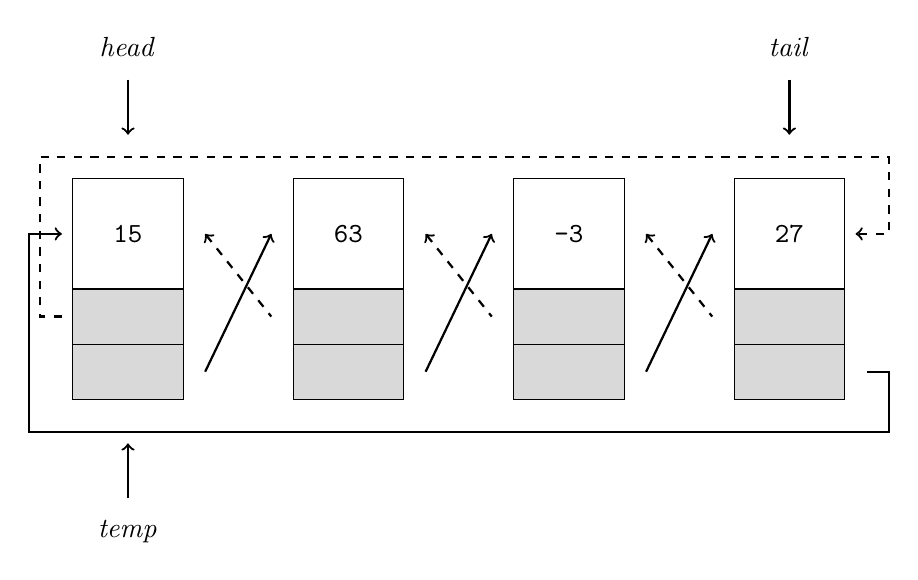
\begin{tikzpicture}[scale=1.4]
        \node[anchor=center] at (0.5, 3.2) {\textit{head}};
        \draw[->,thick] (0.5, 2.9) -- (0.5, 2.4);

        \node[anchor=center] at (6.5, 3.2) {\textit{tail}};
        \draw[->,thick] (6.5, 2.9) -- (6.5, 2.4);

        \node[anchor=center] at (0.5, -1.2) {\textit{temp}};
        \draw[->,thick] (0.5, -0.9) -- (0.5, -0.4);

        \draw[opacity=1,->,thick] (7.2, 0.25) -- (7.4, 0.25) -- (7.4, -0.3) -- (-0.4, -0.3) -- (-0.4, 1.5) -- (-0.1, 1.5);
        \draw[opacity=1,->,thick,dashed] (-0.1, 0.75) -- (-0.3, 0.75) -- (-0.3, 2.2) -- (7.4, 2.2) -- (7.4, 1.5) -- (7.1, 1.5);

%        \draw[->,thick] (7.2, 0.25) -- (7.4, 0.25) -- (7.4, -0.3) -- (1.6, -0.3) -- (1.6, 1.5) -- (1.9, 1.5);
%        \draw[->,thick,dashed] (1.9, 0.75) -- (1.7, 0.75) -- (1.7, 2.2) -- (7.4, 2.2) -- (7.4, 1.5) -- (7.1, 1.5);


        \draw[fill=white] (0,1) rectangle (1,2);
        \draw[fill=gray!30] (0,0) rectangle (1,0.5);
        \draw[fill=gray!30] (0,0.5) rectangle (1,1);
        \node at (0.5,1.5) {\texttt{15}};
        \draw[->,thick] (1.2, 0.25) -- (1.8, 1.5);
        \draw[<-,thick,dashed] (1.2, 1.5) -- (1.8, 0.75);

        \draw[fill=white] (2,1) rectangle (3,2);
        \draw[fill=gray!30] (2,0) rectangle (3,0.5);
        \draw[fill=gray!30] (2,0.5) rectangle (3,1);
        \node at (2.5,1.5) {\texttt{63}};

        \draw[->,thick] (3.2, 0.25) -- (3.8, 1.5);
        \draw[<-,thick,dashed] (3.2, 1.5) -- (3.8, 0.75);

        \draw[fill=white] (4,1) rectangle (5,2);
        \draw[fill=gray!30] (4,0) rectangle (5,0.5);
        \draw[fill=gray!30] (4,0.5) rectangle (5,1);
        \node at (4.5,1.5) {\texttt{-3}};

        \draw[->,thick] (5.2, 0.25) -- (5.8, 1.5);
        \draw[<-,thick,dashed] (5.2, 1.5) -- (5.8, 0.75);

        \draw[fill=white] (6,1) rectangle (7,2);
        \draw[fill=gray!30] (6,0) rectangle (7,0.5);
        \draw[fill=gray!30] (6,0.5) rectangle (7,1);
        \node at (6.5,1.5) {\texttt{27}};

    \end{tikzpicture}

\end{frame}

\begin{frame}[fragile]{Visualização da remoção do início da lista}

    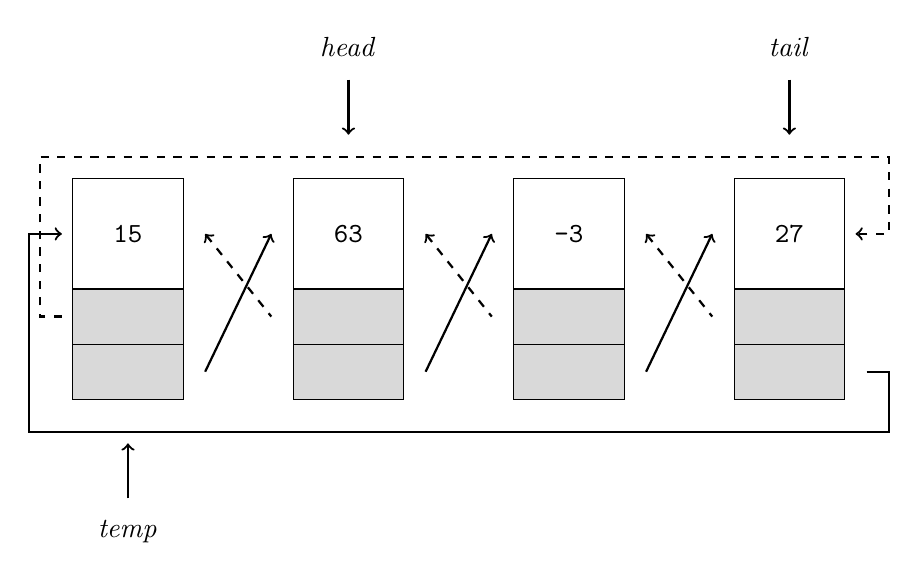
\begin{tikzpicture}[scale=1.4]
        \node[anchor=center] at (2.5, 3.2) {\textit{head}};
        \draw[->,thick] (2.5, 2.9) -- (2.5, 2.4);

        \node[anchor=center] at (6.5, 3.2) {\textit{tail}};
        \draw[->,thick] (6.5, 2.9) -- (6.5, 2.4);

        \node[anchor=center] at (0.5, -1.2) {\textit{temp}};
        \draw[->,thick] (0.5, -0.9) -- (0.5, -0.4);

        \draw[opacity=1,->,thick] (7.2, 0.25) -- (7.4, 0.25) -- (7.4, -0.3) -- (-0.4, -0.3) -- (-0.4, 1.5) -- (-0.1, 1.5);
        \draw[opacity=1,->,thick,dashed] (-0.1, 0.75) -- (-0.3, 0.75) -- (-0.3, 2.2) -- (7.4, 2.2) -- (7.4, 1.5) -- (7.1, 1.5);

%        \draw[->,thick] (7.2, 0.25) -- (7.4, 0.25) -- (7.4, -0.3) -- (1.6, -0.3) -- (1.6, 1.5) -- (1.9, 1.5);
%        \draw[->,thick,dashed] (1.9, 0.75) -- (1.7, 0.75) -- (1.7, 2.2) -- (7.4, 2.2) -- (7.4, 1.5) -- (7.1, 1.5);


        \draw[fill=white] (0,1) rectangle (1,2);
        \draw[fill=gray!30] (0,0) rectangle (1,0.5);
        \draw[fill=gray!30] (0,0.5) rectangle (1,1);
        \node at (0.5,1.5) {\texttt{15}};

        \draw[->,thick] (1.2, 0.25) -- (1.8, 1.5);
        \draw[<-,thick,dashed] (1.2, 1.5) -- (1.8, 0.75);

        \draw[fill=white] (2,1) rectangle (3,2);
        \draw[fill=gray!30] (2,0) rectangle (3,0.5);
        \draw[fill=gray!30] (2,0.5) rectangle (3,1);
        \node at (2.5,1.5) {\texttt{63}};

        \draw[->,thick] (3.2, 0.25) -- (3.8, 1.5);
        \draw[<-,thick,dashed] (3.2, 1.5) -- (3.8, 0.75);

        \draw[fill=white] (4,1) rectangle (5,2);
        \draw[fill=gray!30] (4,0) rectangle (5,0.5);
        \draw[fill=gray!30] (4,0.5) rectangle (5,1);
        \node at (4.5,1.5) {\texttt{-3}};

        \draw[->,thick] (5.2, 0.25) -- (5.8, 1.5);
        \draw[<-,thick,dashed] (5.2, 1.5) -- (5.8, 0.75);

        \draw[fill=white] (6,1) rectangle (7,2);
        \draw[fill=gray!30] (6,0) rectangle (7,0.5);
        \draw[fill=gray!30] (6,0.5) rectangle (7,1);
        \node at (6.5,1.5) {\texttt{27}};

    \end{tikzpicture}

\end{frame}

\begin{frame}[fragile]{Visualização da remoção do início da lista}

    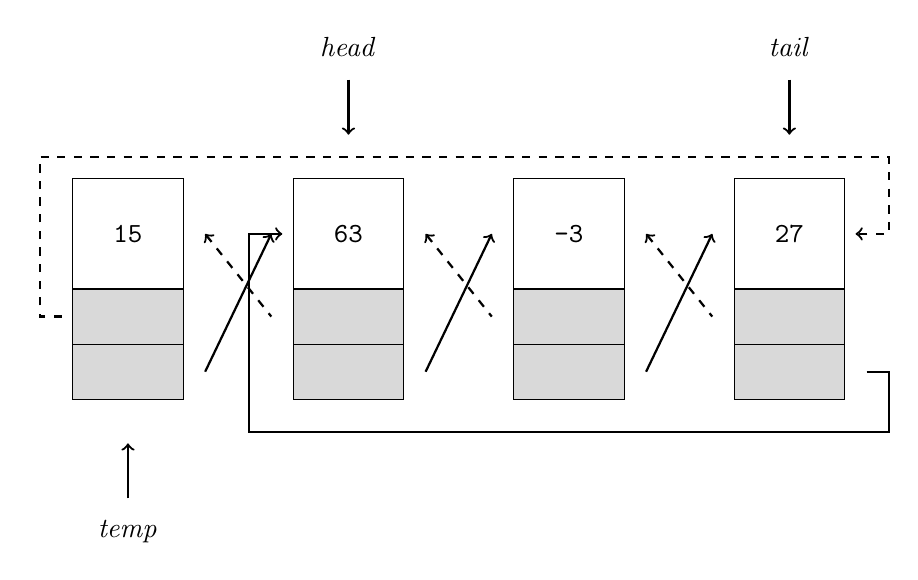
\begin{tikzpicture}[scale=1.4]
        \node[anchor=center] at (2.5, 3.2) {\textit{head}};
        \draw[->,thick] (2.5, 2.9) -- (2.5, 2.4);

        \node[anchor=center] at (6.5, 3.2) {\textit{tail}};
        \draw[->,thick] (6.5, 2.9) -- (6.5, 2.4);

        \node[anchor=center] at (0.5, -1.2) {\textit{temp}};
        \draw[->,thick] (0.5, -0.9) -- (0.5, -0.4);

        \draw[opacity=0,->,thick] (7.2, 0.25) -- (7.4, 0.25) -- (7.4, -0.3) -- (-0.4, -0.3) -- (-0.4, 1.5) -- (-0.1, 1.5);
        \draw[opacity=1,->,thick,dashed] (-0.1, 0.75) -- (-0.3, 0.75) -- (-0.3, 2.2) -- (7.4, 2.2) -- (7.4, 1.5) -- (7.1, 1.5);

        \draw[->,thick] (7.2, 0.25) -- (7.4, 0.25) -- (7.4, -0.3) -- (1.6, -0.3) -- (1.6, 1.5) -- (1.9, 1.5);
%        \draw[->,thick,dashed] (1.9, 0.75) -- (1.7, 0.75) -- (1.7, 2.2) -- (7.4, 2.2) -- (7.4, 1.5) -- (7.1, 1.5);


        \draw[fill=white] (0,1) rectangle (1,2);
        \draw[fill=gray!30] (0,0) rectangle (1,0.5);
        \draw[fill=gray!30] (0,0.5) rectangle (1,1);
        \node at (0.5,1.5) {\texttt{15}};

        \draw[->,thick] (1.2, 0.25) -- (1.8, 1.5);
        \draw[<-,thick,dashed] (1.2, 1.5) -- (1.8, 0.75);

        \draw[fill=white] (2,1) rectangle (3,2);
        \draw[fill=gray!30] (2,0) rectangle (3,0.5);
        \draw[fill=gray!30] (2,0.5) rectangle (3,1);
        \node at (2.5,1.5) {\texttt{63}};

        \draw[->,thick] (3.2, 0.25) -- (3.8, 1.5);
        \draw[<-,thick,dashed] (3.2, 1.5) -- (3.8, 0.75);

        \draw[fill=white] (4,1) rectangle (5,2);
        \draw[fill=gray!30] (4,0) rectangle (5,0.5);
        \draw[fill=gray!30] (4,0.5) rectangle (5,1);
        \node at (4.5,1.5) {\texttt{-3}};

        \draw[->,thick] (5.2, 0.25) -- (5.8, 1.5);
        \draw[<-,thick,dashed] (5.2, 1.5) -- (5.8, 0.75);

        \draw[fill=white] (6,1) rectangle (7,2);
        \draw[fill=gray!30] (6,0) rectangle (7,0.5);
        \draw[fill=gray!30] (6,0.5) rectangle (7,1);
        \node at (6.5,1.5) {\texttt{27}};

    \end{tikzpicture}

\end{frame}

\begin{frame}[fragile]{Visualização da remoção do início da lista}

    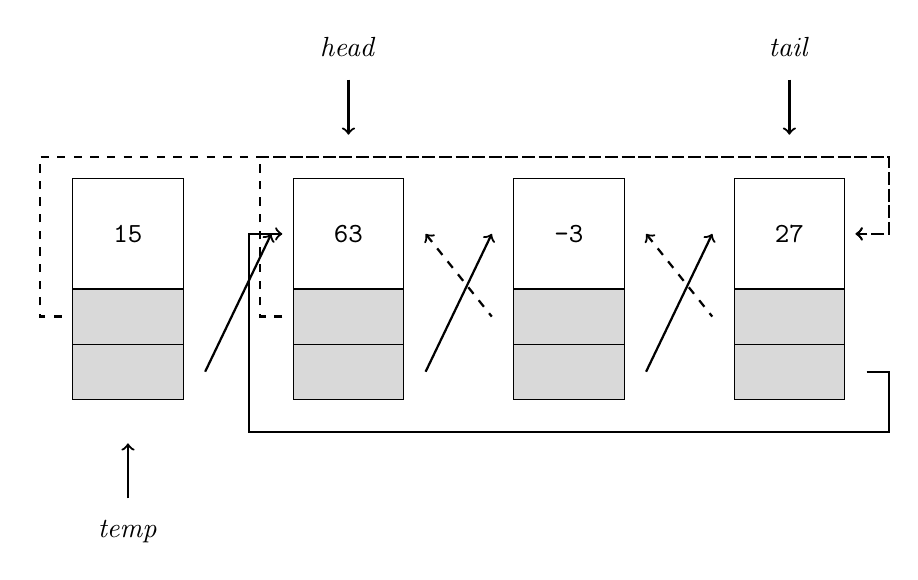
\begin{tikzpicture}[scale=1.4]
        \node[anchor=center] at (2.5, 3.2) {\textit{head}};
        \draw[->,thick] (2.5, 2.9) -- (2.5, 2.4);

        \node[anchor=center] at (6.5, 3.2) {\textit{tail}};
        \draw[->,thick] (6.5, 2.9) -- (6.5, 2.4);

        \node[anchor=center] at (0.5, -1.2) {\textit{temp}};
        \draw[->,thick] (0.5, -0.9) -- (0.5, -0.4);

        \draw[opacity=0,->,thick] (7.2, 0.25) -- (7.4, 0.25) -- (7.4, -0.3) -- (-0.4, -0.3) -- (-0.4, 1.5) -- (-0.1, 1.5);
        \draw[opacity=1,->,thick,dashed] (-0.1, 0.75) -- (-0.3, 0.75) -- (-0.3, 2.2) -- (7.4, 2.2) -- (7.4, 1.5) -- (7.1, 1.5);

        \draw[->,thick] (7.2, 0.25) -- (7.4, 0.25) -- (7.4, -0.3) -- (1.6, -0.3) -- (1.6, 1.5) -- (1.9, 1.5);
        \draw[->,thick,dashed] (1.9, 0.75) -- (1.7, 0.75) -- (1.7, 2.2) -- (7.4, 2.2) -- (7.4, 1.5) -- (7.1, 1.5);


        \draw[fill=white] (0,1) rectangle (1,2);
        \draw[fill=gray!30] (0,0) rectangle (1,0.5);
        \draw[fill=gray!30] (0,0.5) rectangle (1,1);
        \node at (0.5,1.5) {\texttt{15}};

        \draw[->,thick] (1.2, 0.25) -- (1.8, 1.5);
%        \draw[<-,thick,dashed] (1.2, 1.5) -- (1.8, 0.75);

        \draw[fill=white] (2,1) rectangle (3,2);
        \draw[fill=gray!30] (2,0) rectangle (3,0.5);
        \draw[fill=gray!30] (2,0.5) rectangle (3,1);
        \node at (2.5,1.5) {\texttt{63}};

        \draw[->,thick] (3.2, 0.25) -- (3.8, 1.5);
        \draw[<-,thick,dashed] (3.2, 1.5) -- (3.8, 0.75);

        \draw[fill=white] (4,1) rectangle (5,2);
        \draw[fill=gray!30] (4,0) rectangle (5,0.5);
        \draw[fill=gray!30] (4,0.5) rectangle (5,1);
        \node at (4.5,1.5) {\texttt{-3}};

        \draw[->,thick] (5.2, 0.25) -- (5.8, 1.5);
        \draw[<-,thick,dashed] (5.2, 1.5) -- (5.8, 0.75);

        \draw[fill=white] (6,1) rectangle (7,2);
        \draw[fill=gray!30] (6,0) rectangle (7,0.5);
        \draw[fill=gray!30] (6,0.5) rectangle (7,1);
        \node at (6.5,1.5) {\texttt{27}};

    \end{tikzpicture}

\end{frame}

\begin{frame}[fragile]{Visualização da remoção do início da lista}

    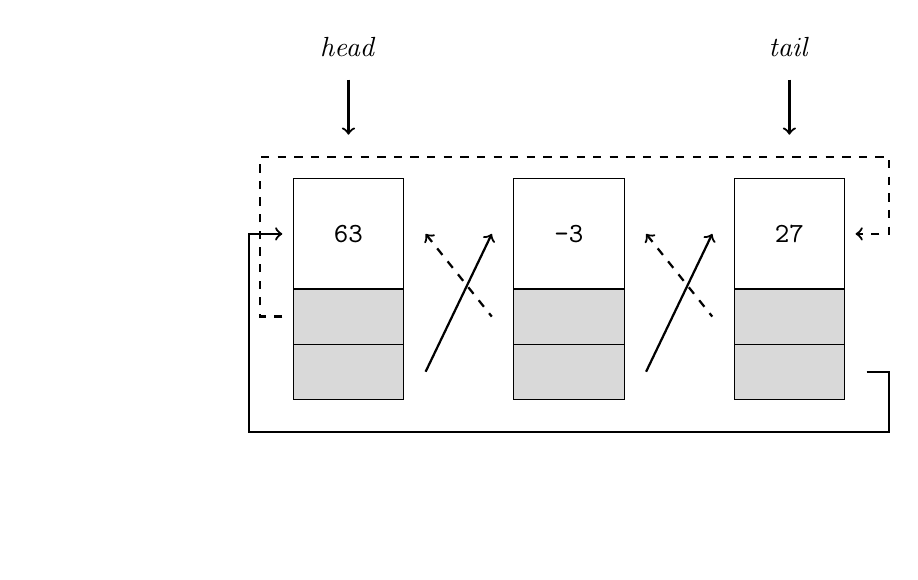
\begin{tikzpicture}[scale=1.4]
        \node[anchor=center] at (2.5, 3.2) {\textit{head}};
        \draw[->,thick] (2.5, 2.9) -- (2.5, 2.4);

        \node[anchor=center] at (6.5, 3.2) {\textit{tail}};
        \draw[->,thick] (6.5, 2.9) -- (6.5, 2.4);

        \node[opacity=0,anchor=center] at (0.5, -1.2) {\textit{temp}};
        \draw[opacity=0,->,thick] (0.5, -0.9) -- (0.5, -0.4);

        \draw[opacity=0,->,thick] (7.2, 0.25) -- (7.4, 0.25) -- (7.4, -0.3) -- (-0.4, -0.3) -- (-0.4, 1.5) -- (-0.1, 1.5);
        \draw[opacity=0,->,thick,dashed] (-0.1, 0.75) -- (-0.3, 0.75) -- (-0.3, 2.2) -- (7.4, 2.2) -- (7.4, 1.5) -- (7.1, 1.5);

        \draw[->,thick] (7.2, 0.25) -- (7.4, 0.25) -- (7.4, -0.3) -- (1.6, -0.3) -- (1.6, 1.5) -- (1.9, 1.5);
        \draw[->,thick,dashed] (1.9, 0.75) -- (1.7, 0.75) -- (1.7, 2.2) -- (7.4, 2.2) -- (7.4, 1.5) -- (7.1, 1.5);


        \draw[opacity=0,fill=white] (0,1) rectangle (1,2);
%        \draw[fill=gray!30] (0,0) rectangle (1,0.5);
%        \draw[fill=gray!30] (0,0.5) rectangle (1,1);
%        \node at (0.5,1.5) {\texttt{15}};

%        \draw[->,thick] (1.2, 0.25) -- (1.8, 1.5);
%        \draw[<-,thick,dashed] (1.2, 1.5) -- (1.8, 0.75);

        \draw[fill=white] (2,1) rectangle (3,2);
        \draw[fill=gray!30] (2,0) rectangle (3,0.5);
        \draw[fill=gray!30] (2,0.5) rectangle (3,1);
        \node at (2.5,1.5) {\texttt{63}};

        \draw[->,thick] (3.2, 0.25) -- (3.8, 1.5);
        \draw[<-,thick,dashed] (3.2, 1.5) -- (3.8, 0.75);

        \draw[fill=white] (4,1) rectangle (5,2);
        \draw[fill=gray!30] (4,0) rectangle (5,0.5);
        \draw[fill=gray!30] (4,0.5) rectangle (5,1);
        \node at (4.5,1.5) {\texttt{-3}};

        \draw[->,thick] (5.2, 0.25) -- (5.8, 1.5);
        \draw[<-,thick,dashed] (5.2, 1.5) -- (5.8, 0.75);

        \draw[fill=white] (6,1) rectangle (7,2);
        \draw[fill=gray!30] (6,0) rectangle (7,0.5);
        \draw[fill=gray!30] (6,0.5) rectangle (7,1);
        \node at (6.5,1.5) {\texttt{27}};

    \end{tikzpicture}

\end{frame}

\begin{frame}[fragile]{Implementação da remoção do início}
    \inputsnippet{c++}{155}{166}{circular_list.h}
\end{frame}

\begin{frame}[fragile]{Remoção do final da lista}

    \begin{itemize}
        \item A remoção do último elemento de uma lista
            circular (\code{c++}{pop_back()}) tem complexidade $O(1)$

        \item Efetivamente, ela pode ser reduzida à uma remoção do início: basta delocar tanto
            \code{c}{head} quanto \code{c}{tail} uma posição para trás

        \item Esta simplificação evita a duplicidade de código, e mantém os invariantes da lista
    \end{itemize}

\end{frame}

\begin{frame}[fragile]{Implementação da remoção do final}
    \inputsnippet{c++}{168}{180}{circular_list.h}
\end{frame}

\begin{frame}[fragile]{Remoção em posição arbitrária}

    \begin{itemize}
        \item A remoção em posição arbitrária também tem complexidade $O(1)$ ou $O(N)$, 
            caso esteja disponível ou não um ponteiro para o elemento a ser removido

        \item Novamente é possível reduzir este problema para o da remoção do início: basta
            avançar \code{c}{head} e \code{c}{tail} simultaneamente até que \code{c}{head} se
            iguale com o ponteiro do elemento a ser removido

        \item Assim como nas demais remoções, a tentativa de excluir um elemento de uma lista
            vazia constitui um erro
    \end{itemize}

\end{frame}

\begin{frame}[fragile]{Exemplo de uso da lista encadeada}
    \inputsnippet{c++}{1}{20}{main.cpp}
\end{frame}

\begin{frame}[fragile]{Exemplo de uso da lista encadeada}
    \inputsnippet{c++}{21}{41}{main.cpp}
\end{frame}
